%! Author = adnansiddiquei
%! Date = 05/03/2024

% Preamble
\documentclass[a4paper,11pt]{article}
\pdfoutput=1

% Packages
\usepackage{jcappub}
\usepackage[T1]{fontenc}
\usepackage{listings}
\usepackage{roboto}
\usepackage{subcaption}
\usepackage{blindtext}
\usepackage{float}

\newcommand{\inlinecode}[1]{\lstinline{#1}}
\lstset{basicstyle=\fontfamily{pcr}\selectfont}


\title{\boldmath C2: Advanced Research Computing - Coursework Assignment}

% %simple case: 2 authors, same institution
\author{Adnan Siddiquei}
\affiliation{University of Cambridge}

% e-mail addresses: one for each author, in the same order as the authors
\emailAdd{as3438@cam.ac.uk}
\note{Word Count: 2857 (including figure captions and appendix.)}


\begin{document}
\maketitle
\flushbottom


%! Author = adnansiddiquei
%! Date = 05/03/2024

\section{Introduction}\label{sec:intro}
    Conway's Game of Life...

%! Author = adnansiddiquei
%! Date = 08/03/2024

\section{Selection of Solution Algorithm and Prototyping}\label{sec:prototyping}
    \begin{figure}[htb]
    \centering
    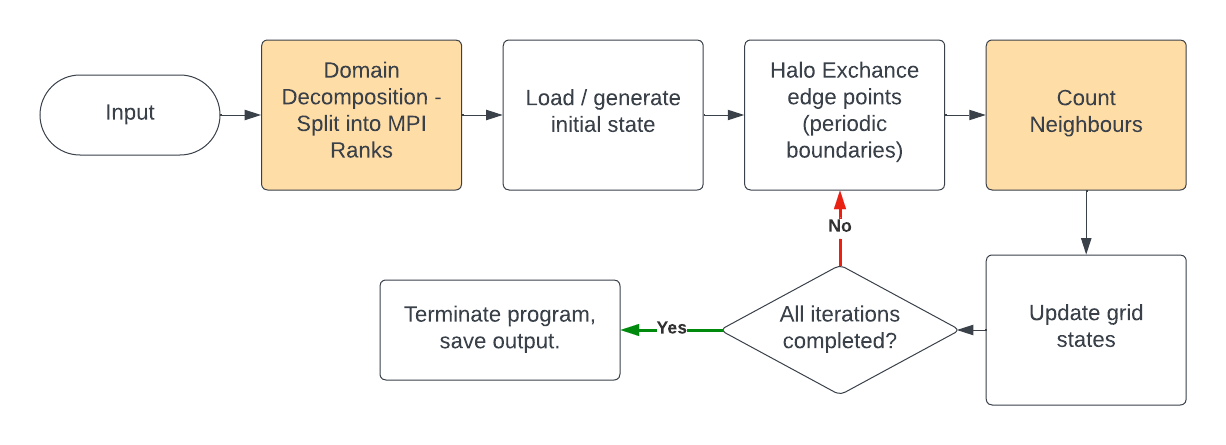
\includegraphics[width=0.9\textwidth]{./figures/high-level-flowchart}
    \caption{A high-level flow chart depicting the algorithm. The key points for efficiency considerations
    are highlighted in red, the considerations are discussed in the main text.}
    \label{fig:high-level-flowchart}
    \end{figure}

    Fig.\eqref{fig:high-level-flowchart} shows the high-level algorithm being used to simulate Conway's
    Game of Life.
    The key points of consideration with regard to performance are highlighted in red.
    There are 3 domain decomposition methods available (column, row and block decomposition) as well as multiple
    ways to count neighbours and update grid states.
    As indicated in Fig.\eqref{fig:high-level-flowchart}, communication overheads between MPI ranks can be hidden
    behind computation by using non-blocking communication and counting whichever neighbours are available at the time.
    Likewise, the actual method of counting neighbours and updating the grid can be done in a variety of ways, each with
    their own merits.
    All these considerations are discussed thoroughly in this section, and then they are investigated in the next
    section.

    \subsection{Domain Decomposition and Neighbour Counting Algorithm}\label{subsec:domain-decomp}
    Domain decomposition can be done by either strips or blocks.
    Strips has the advantage that it is simpler to implement but will have more memory needing to be passed between
    boundaries, with the opposite being true for blocks.
    Therefore, the choice of domain decomposition will need to be tested to see which is more efficient as the data
    size and number of MPI ranks increases.
    However, the overheads of communication can be effectively nullified if the communication is hidden behind computation,
    as such, this also needs to be explored to see what proportion of the communication can be hidden.

    The neighbour counting algorithm has 2 possible implementations, a simple convolution and a separable kernel.
    \begin{itemize}
        \item \textbf{Simple convolution.} Loop through each cell, and count the number of neighbours.
            This is equivalent to a 3x3 convolution with the below kernel.
            \begin{equation}
            \begin{bmatrix}
            1 & 1 & 1 \\
            1 & 0 & 1 \\
            1 & 1 & 1 \\
            \end{bmatrix}\label{eq:kernel1}
            \end{equation}
            This requires a total of $8N^{2}$ addition operations (the $9N^{2}$ multiplication operations that would usually occur can
            be ignored because the kernel only contain 1s and 0s so we can skip the multiplication operation in this special case).
        \item \textbf{Separable kernel.} If the following kernel is used instead,
            \begin{equation}
            \begin{bmatrix}
            1 & 1 & 1 \\
            1 & 1 & 1 \\
            1 & 1 & 1 \\
            \end{bmatrix}\label{eq:kernel2}
            \end{equation}
            then the kernel becomes separable.
            This means that the kernel can be split into two 1D identical kernels \(\begin{bmatrix} 1 & 1 & 1 \end{bmatrix}\) and
            applied in two passes which yields $2N^{2}$ addition operations per pass, yielding a total of $4N^{2}$ operations \cite{separable-kernel}.
            After another ${N^{2}}$ addition operations, to correct for replacing the central 0 with a 1, the total number of
            operations becomes $5N^{2}$.
            Therefore, the separable kernel method yields a theoretical speedup of $8/5 \approx 1.6$.
            However, due to strided memory access on the vertical pass, the speedup will be less than this.
            Although, the vertical pass can be made more efficient by transposing the grid and making the data contiguous,
            it will need to be investigated whether the additional overhead of transposing the grid yields any speedup.
    \end{itemize}

    The simple convolution method would prefer column-wise decomposition as it would reduce the number of cache misses
    when counting the 6 neighbours that are not horizontally adjacent to the current cell.
    This is because shorter rows would reduce the distance in memory between a cell and it's vertical neighbour.
    Theoretically, the separable kernel should not have this issue if the separable convolution can be applied in two horizontal
    passes with a transpose in between.

    \subsection{Hiding Communication Behind Computation}\label{subsec:hiding-comms}
    To the extent of hiding communication behind computation, the separable convolution allows naturally for the horizontal
    pass to be done first, and then the vertical pass to be done after the vertical halos have been exchanged.
    Doing the vertical pass first is also possible but likely to be less efficient due to the strided memory access (assuming
    the grid is represented as 1D array in row-major order).
    This method, however, would only hide communication if the horizontal halos arrive before the vertical halos which is
    only guaranteed (or with sufficiently higher probability) in row-based decomposition where the horizontal halos live
    on the same MPI rank.
    For column based decomposition it is unlikely that the large chunk of non-contiguous data (horizontal column borders)
    will arrive before the smaller chunk of contiguous data (vertical row borders) within the same MPI rank.
    For block decomposition, there would be many factors involved such as the physical positioning of the MPI ranks and the network
    topology which would affect the communication overheads between MPI ranks.

    The alternative option for hiding communication is to count the neighbours with the simple convolution
    for all the cells that are not on the boundary, and then count the neighbours for the cells on the boundary once the halo
    exchange has been completed (note, this method is later referred back to as the 'SimpleIO' method as a short form for
    'Simple Inner Outer' method).
    This removes the dependency on certain halos arriving before others, but downside of this is that it involves a lot
    of non-contiguous memory access (when doing the outer loop), which is not ideal for performance, but how this method
    compares to the previous method as the simulation scaled will need to be investigated.

    It is worth noting that similar inner-outer method can be applied to the separable kernel method, where the horizontal
    pass is done first while excluding the left and right most columns until the left and right halos have arrived.

    \subsection{Updating Grid}\label{subsec:update-grid}
    Given the neighbour count and the current state of the grid, there are a few possible ways to update the grid \cite{branchless-programming}.
    \begin{itemize}
        \item \textbf{\inlinecode{if} statements.} This is the most straightforward implementation.
        The minimum number of \inlinecode{if} statements required to implement the rules of Conway's Game of Life is 3,
        and it is unlikely the CPU will be able to optimise this to any degree with branch prediction, so
        this method will likely be the slowest.
        \item \textbf{Bitwise operations.} This method removes all \inlinecode{if} statements and replaces them with
            inline bitwise (\inlinecode{&&} and \inlinecode{||}) operations.
        \item \textbf{Lookup table.} Given that there is only 18 states a cell can be in (dead or alive, with 0 to 8 neighbours),
            a lookup array can be used to update the grid with the new state of each cell, given one of the current
            18 states.
    \end{itemize}
    The efficacy of these methods will need to be tested to see which is the most efficient.

    \subsection{OpenMP with MPI}\label{subsec:omp-with-mpi}
    The final consideration is to assess how to use OpenMP with MPI.
    Not all loops will be infinitely parallelisable, more threads won't always yield a linear speedup.
    Likewise, more MPI ranks yields more communication overheads, and as such there will be trade-offs in this respect.
    The trade-off between OpenMP and MPI will need to be investigated empirically to see what the best combination is.




%! Author = adnansiddiquei
%! Date = 08/03/2024

\section{Development}\label{sec:development}
    This section discusses the development of the code and software engineering best practises.

    CMake was used to manage the entire build process, including the compilation of the code, and running of tests.
    For formatting, the code was run through \inlinecode{clang-format} automatically on every build to ensure a consistent
    style.
    This was done by writing a custom CMake function (based off J.R. Fergusson's template) and tying it into the build process.

    Tests were written using the GoogleTest framework, and tied into the build process using CMake.
    These tests were run regularly, primarily before creating any merge requests into main.
    To make writing the tests easy, and to ensure that the tests were comprehensive, the code was written in a modular
    way, such that the code was easy to test in small isolated units.

    Generally, best practises with regard to Git were followed, such as creating a new branch for every new feature
    or bug fix, and writing meaningful commit messages.
    New issues were created for every feature, and branches and merge requests were made against these issues to make
    work easy to track.

    Additionally, the code was documented using Doxygen to ensure that the code was easy to understand and maintain.
    This was particularly important as aspects of the code were quite complex.

    Polymrphism was also used to make the code more modular and easier to maintain.
    Much of the utility code is written in a generic manner and then inherited by the specific classes that need it.
    For example, the \inlinecode{Array2D} acted as a base class for the \inlinecode{Array2DWithHalo} which further
    acted as a base class for \inlinecode{ConwaysArray2DWithHalo}.
    This allowed for the code to be kept minimal and reusable.

    Effective error handling was also implemented, raising descriptive errors where possible, especially against
    invalid user input.


%! Author = adnansiddiquei
%! Date = 08/03/2024

\section{Experimentation, Profiling and Optimisation}\label{sec:profiling}
\begin{figure}[t]
\centering
\begin{subfigure}{0.9\textwidth}
  \centering
  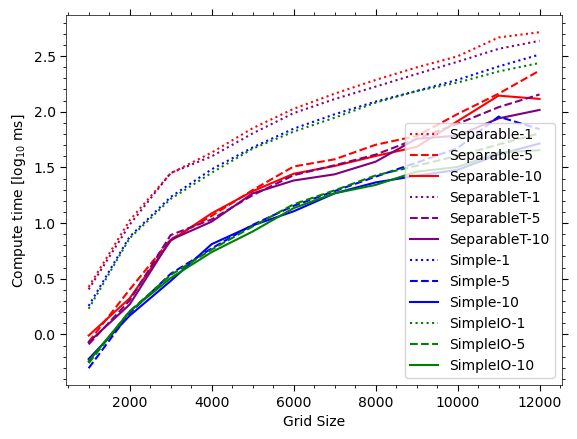
\includegraphics[width=.8\linewidth]{./figures/convolutions}
  \caption{A figure showing the compute time for 4 of the convolution methods for counting neighbours.
        The colour of the line indicates the method used, and the line style (dotted, dashed, solid) indicates the number
        OpenMP threads used (1, 5 and 10 respectively).
        Only 1 MPI rank was used.
        The x-axis shows the size of one dimension of the square grid.
        The Simple and Separable methods are as described in \eqref{subsec:domain-decomp} and the SimpleIO method is
        as described in \eqref{subsec:hiding-comms})
        The SeparableT method is the Separable method done in 2 horizontal passes with a transpose in between, except
        the time on the graph is just the compute time to repeat the first horizontal pass twice (for simplicity).}
  \label{fig:convolutions}
\end{subfigure}%
\hfill
\begin{subfigure}{0.9\textwidth}
  \centering
  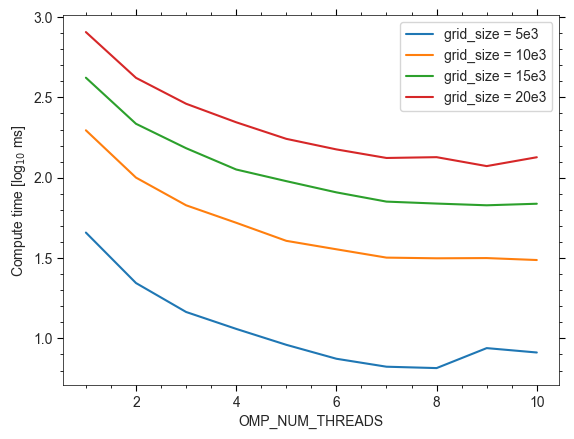
\includegraphics[width=0.8\linewidth]{./figures/simpleio}
  \caption{A figure showing how the compute time varies for the SimpleIO method as the number of OMP threads is changed.
    1 MPI rank was used, and compute time was averaged over 3 runs.}
  \label{fig:simpleio}
\end{subfigure}
\caption{Performance testing results for the various convolution methods for counting neighbours.}
\label{fig:conv}
\end{figure}

\begin{figure}[t]
\centering
\begin{subfigure}{0.9\textwidth}
  \centering
  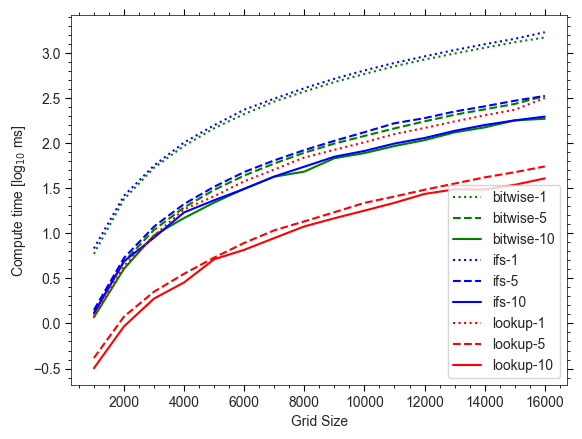
\includegraphics[width=.8\linewidth]{./figures/transitions}
  \caption{A figure showing the compute time (the time taken to update the entire grid once) for the 3 the update methods
    discussed in Section \eqref{subsec:update-grid}.
    The colour of the line indicates the method used, and the line style (dotted, dashed, solid) indicates the number
    OpenMP threads used (1, 5 and 10 respectively).
    Only 1 MPI rank was used and the compute time was averaged over 3 runs.}
  \label{fig:transitions}
\end{subfigure}%
\hfill
\begin{subfigure}{0.9\textwidth}
  \centering
  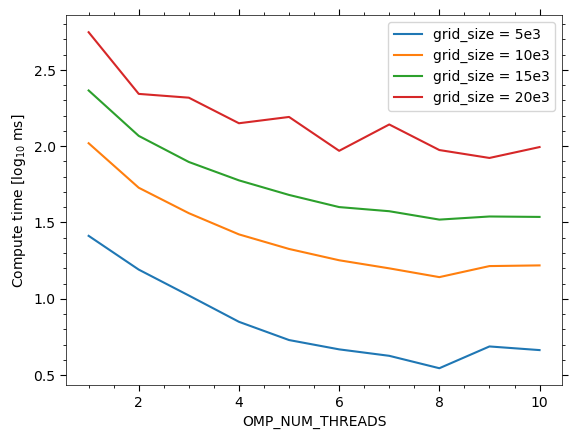
\includegraphics[width=0.8\linewidth]{./figures/lookup}
  \caption{A figure showing how the compute time varies for the updating the grid using the lookup method as the number
    of OMP threads is changed.
    1 MPI rank was used, and compute time was averaged over 5 runs.}
  \label{fig:lookup}
\end{subfigure}
\caption{Performance testing results for the various convolution methods for counting neighbours.}
\label{fig:trans}
\end{figure}

\begin{figure}[t]
\centering
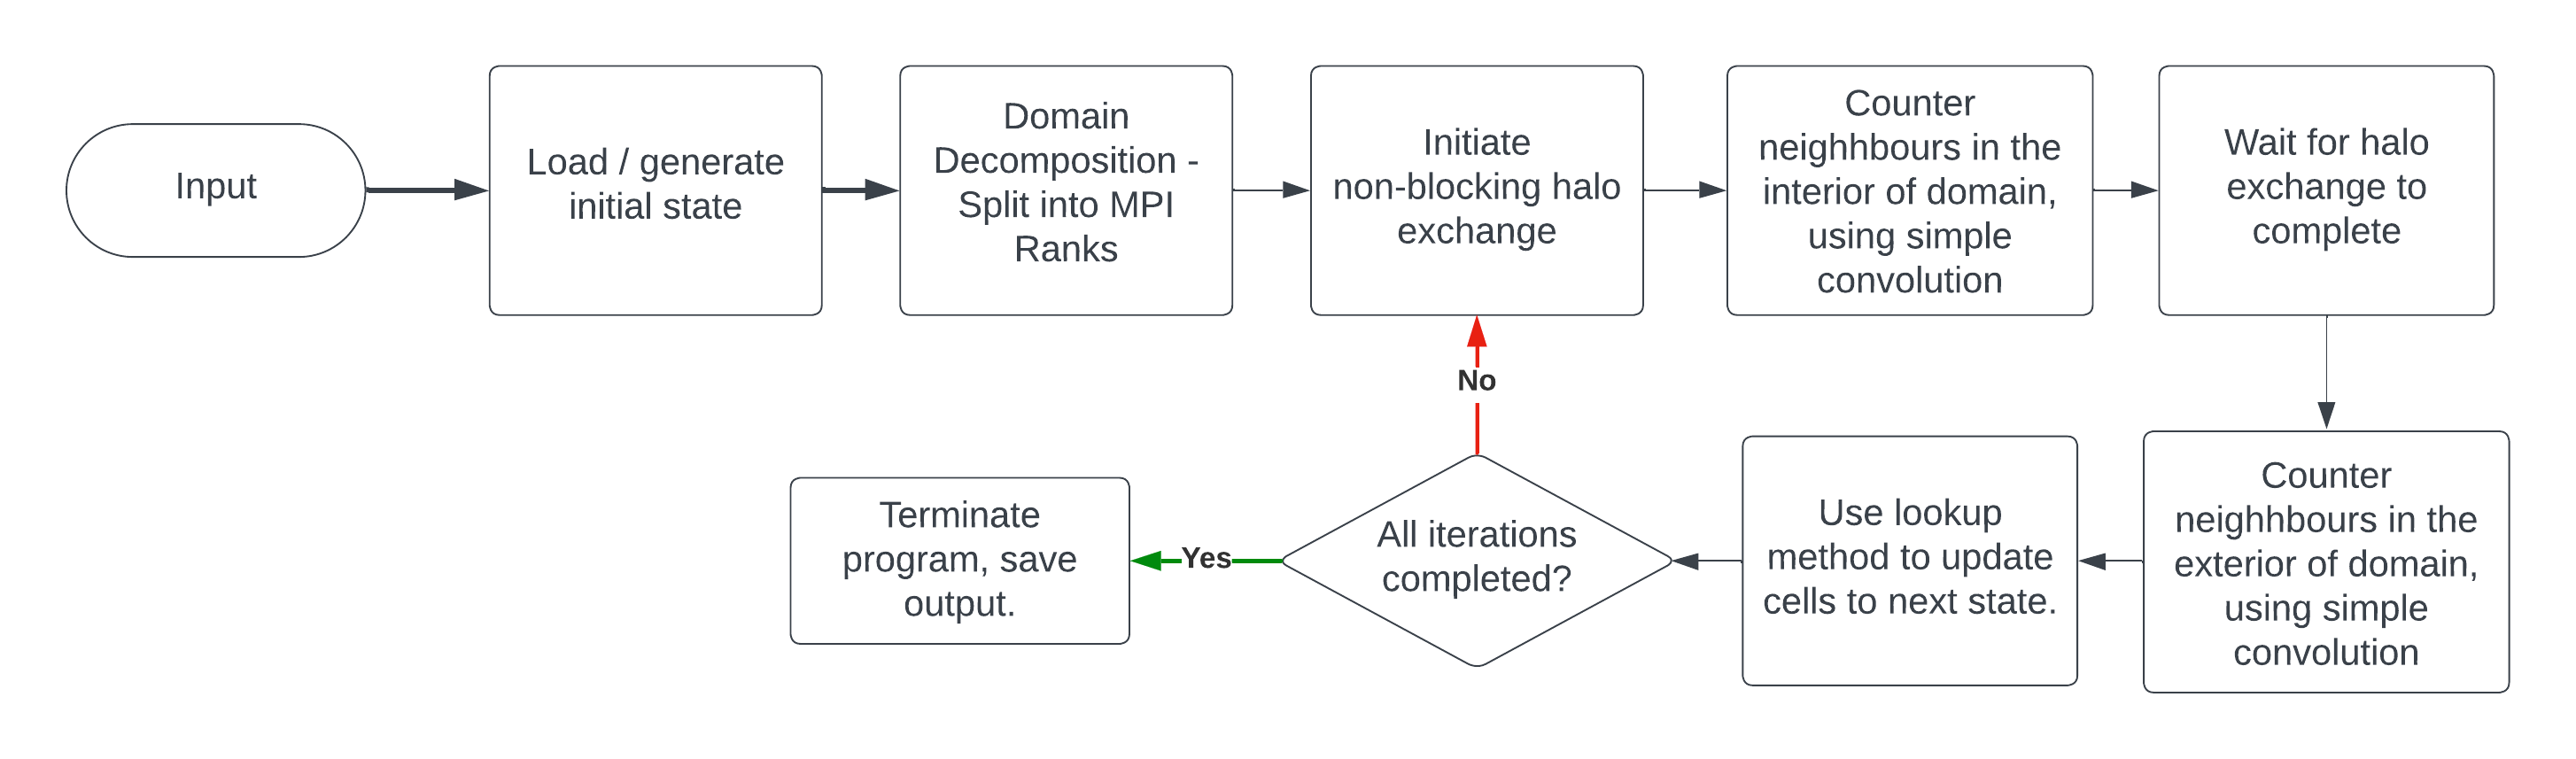
\includegraphics[width=0.85\textwidth]{./figures/flowchat-2}
\caption{An updated version of Fig.\eqref{fig:high-level-flowchart} with the conclusions from the experimentation
and profiling.}
\label{fig:flowhcart-2}
\end{figure}

\begin{figure}[t]
\centering
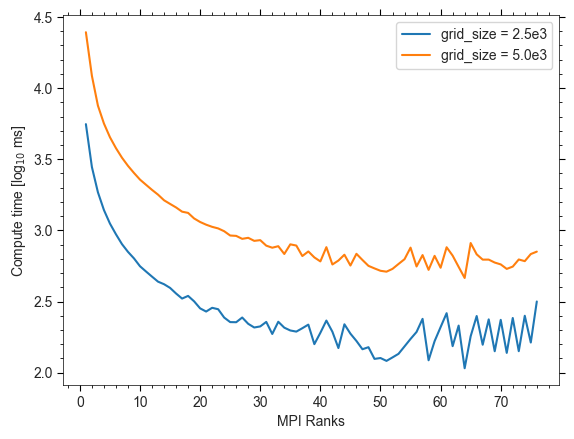
\includegraphics[width=0.9\textwidth]{./figures/mpi_hpc}
\caption{A plot of the compute time for the full simulation on a singular Icelake node (76 cores).
    The number of MPI ranks was varied but the OMP thread count was kept at 1.
    The compute time was averaged over 2 runs for grid sizes of $5 \times 10^{3}$ and $2.5 \times 10^{3}$ as they evolved
    over 200 generations.}
\label{fig:mpi_hpc}
\end{figure}

\begin{figure}[t]
\centering
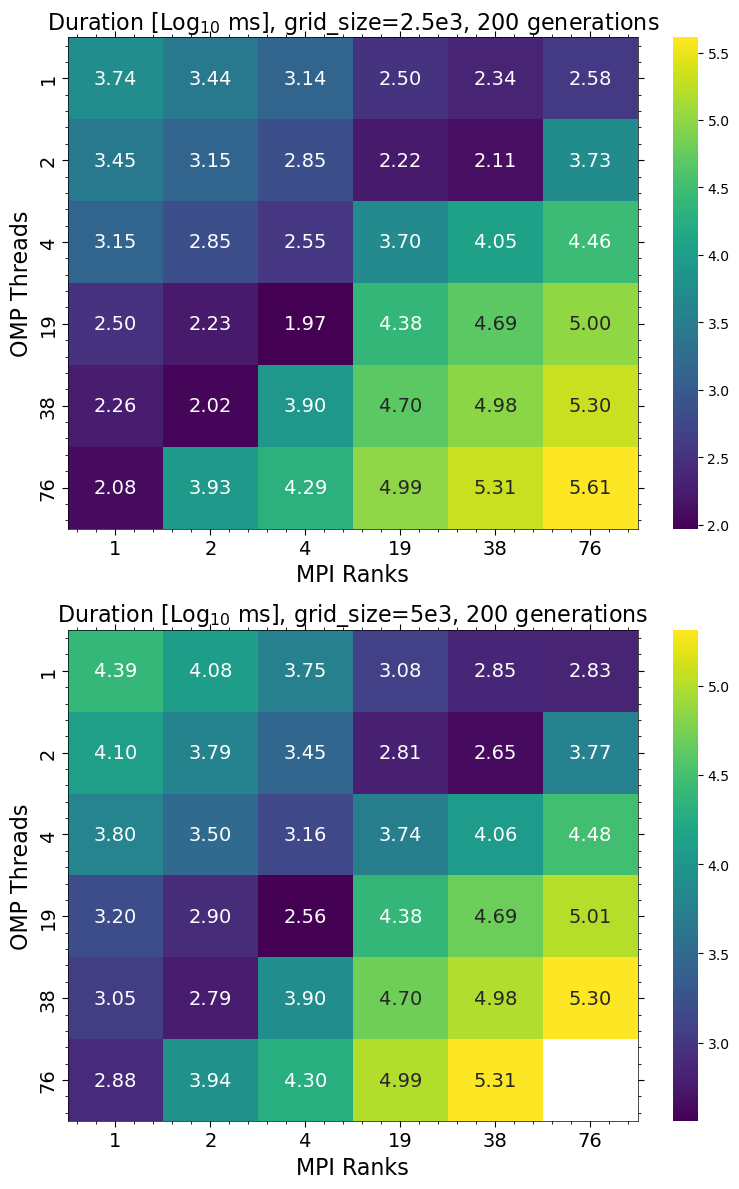
\includegraphics[width=0.8\textwidth]{./figures/mpi_vs_omp_hpc}
\caption{Heatmaps of the $Log_{10}(duration)$ for the full simulation on a singular Icelake node (76 cores).
    Both the number of MPI ranks and OMP threads were varied, with the diagonal (going from the bottom left to the top right)
    representing the full usage configurations of the node (where the number of MPI ranks and OMP threads multiplied to 76).
    The compute time was averaged over 2 runs}
\label{fig:mpi_vs_omp_hpc}
\end{figure}

This section discusses the experimentation and profiling of the different methods discussed in Section \eqref{sec:prototyping}.
Experimentation to decide algorithmic choices (which convolution Section~\eqref{subsec:domain-decomp}, and update method
Section~\eqref{subsec:update-grid} to use) was done on a Macbook M1 Pro (see Appendix~\eqref{app:macbook-specs} for specs).
Following the implementation of these decisions, the optimal algorithm was tested on a singular Icelake node to determine
the optimal number of MPI ranks and OMP threads to use for the full simulation.

\subsection{Profiling the Convolution Methods}\label{subsec:prof-conv}
Fig.\eqref{fig:convolutions} shows the compute time across 4 different convolution methods for counting neighbours
and how they scale with \inlinecode{grid_size} and \inlinecode{OMP_NUM_THREADS}.
The first observation is that both the simple methods are faster than both of the separable methods, which is
at face value, unexpected.
Furthermore, there is a negligible difference in speed between the Simple and SimpleIO method which is a positive
outcome which means the SimpleIO method is a good candidate for hiding communication overheads, as the vast majority
of the computation can be done while waiting for the communication to complete.
OpenMP was used to parallelise the convolution methods, as such, the Figure illustrates the compute times for a variety
of thread counts.

Loop unrolling was implemented in all of these convolutions, the kernel was applied
to the grid manually rather than having an additional loop (0 to 8) which applied the kernel.
Experimentally, this was found to yield about a 2.5x speedup (for the sake of brevity, no figures were generated to
supplement this conclusion).
Additionally, all of the double nested loops (which looped over the rows and columns of the grids) were parallelised
using the OMP \inlinecode{parallel for collapse} clause which allowed OMP to collapse and parallelise the
nested loops.

Fig.\eqref{fig:simpleio} illustrates how the SimpleIO method parallelises as the thread count is increased.
As expected, it shows diminishing returns, with the compute time flattening out as the thread count increases.

\subsection{Profiling the Update Methods}\label{subsec:prof-trans}
Fig.\eqref{fig:transitions} explores the update methods discussed in Section \eqref{subsec:update-grid}, with a
clear conclusion that the lookup method is the fastest, and as expected, the \inlinecode{if} method is the slowest.
This makes sense, due to the (effectively) random nature of the simulation, the CPU will have little success
in branch predictions, contributing to the slowness of the \inlinecode{if} method.
The frequent lookup in an 18-length array is relatively inexpensive compared to frequent branching.

Similar to Fig.\eqref{fig:simpleio}, Fig.\eqref{fig:lookup} shows that the lookup method for updating the grid starts
to show diminishing returns in performance after about 8 OMP threads have been created.

\subsection{Algorithm Conclusions}\label{subsec:interim-conclusions}
Given the above results, the SimpleIO and lookup methods are the best candidates for the neighbour counting and grid
updating algorithms respectively.
The SimpleIO can be used to hide communication overheads effectively and the lookup method is the fastest way to
update the grid, Fig~\eqref{fig:flowhcart-2} shows an updated flowchart of the overall algorithm.
These conclusions are likely transferable to other architectures (although the exact relative speed differences will
likely differ from chip to chip), and so these conclusions were not re-evaluated on the Icelake node.
It is likely that for the M1 Pro, the bottleneck at roughly 8 OMP threads is due to memory constraints rather
than the algorithm itself not parallelising well, given that the datasets used in the simulation are large enough
to completely fill L1 and shared L2 caches.

Additionally, the optimal domain decomposition was not explored due to time constraints, row-wise decomposition was implemented
for the sake of simplicity and it was preferred over column-wise decomposition to reduce non-contiguous data transfer
in the halo exchange.

\subsection{MPI Ranks and OMP Threads}\label{subsec:mpi-omp}
With the conclusions from Section~\eqref{subsec:interim-conclusions} implemented this section explores the dynamic of
the number of MPI ranks and OMP threads on the compute time.

Fig.\eqref{fig:mpi_hpc} shows the compute time for the full simulation on a singular Icelake node as the number of MPI
ranks is varied.
The compute time sharply decreases as the number of MPI ranks is increased, but tapers off at around 40 MPI ranks,
yielding diminishing returns following this point.
Figure~\eqref{fig:mpi_vs_omp_hpc} takes this analysis further and plots a heatmap of the compute time for the full
simulation as the number of MPI ranks and OMP threads are both varied.
As expected, generally the best performance was achieved on the full usage diagonal of the heatmap, where the number of
MPI ranks and OMP threads multiplied to 76 (the number of cores on the Icelake node), with an interesting exception at
19 ranks with 4 threads.
Another observation is that upper left triangle is preferred over the lower right triangle, i.e.,
configurations resulting in under-utilisation of the node were preferred over configurations resulting in over-utilisation
(hyper-threading).
This is likely due to the overheads of managing additional threads and ranks.
In fact, almost identical performance is seen across both grid sizes in the over-utilisation region.
The compute times in this region are a whole 2 magnitudes larger than the compute times in the full usage region indicating
the effects of too many ranks and threads.

There was, however, a consistent winner across both grid sizes and this was the 4 rank and 19 thread configuration.









%! Author = adnansiddiquei
%! Date = 08/03/2024

\section{Conclusion}\label{sec:conclusion}
In this report, the performance of various algorithms to implement Conway's Game of Life was investigated.
Algorithms for neighbour counting and grid updating were discussed, and the performance of each was tested, arriving at
the conclusion that for this specific implementation, the simple convolution and lookup methods were the most efficient
for neighbour counting and grid updating respectively.
Furthermore, full grid-wise search of MPI rank and OMP thread combinations was performed on the Icelake node, and the best
performing combination found was 4 ranks with 19 nodes.








\clearpage
\appendix

\section{Macbook M1 Pro Chip Specifications}\label{app:macbook-specs}
The M1 pro chip has \cite{apple-m1}:
\begin{itemize}
    \item 10 cores; 8 high-performance cores and 2 high-efficiency cores;
    \item Performance cores have 192KB + 128KB L1 instruction + data cache;
    \item Efficiency cores have 128KB + 64KB L1 instruction + data cache;
    \item L1 line size is 64 bytes;
    \item The 8 high-performance cores are divided into 2 clusters, each cluster sharing a 12MB L2 cache;
    \item The 2 high-efficiency cores share a 4MB L2 cache;
    \item 16GB RAM;
\end{itemize}



\begin{thebibliography}{99}

\bibitem{separable-kernel}
Steve Eddins,
\textit{Steve on Image Processing with MATLAB}.
Available at: \url{https://blogs.mathworks.com/steve/2006/10/04/separable-convolution/}
[Accessed: 8-Mar-2024].

\bibitem{branchless-programming}
Srdjan Delić,
\textit{Branchless programming — Why your CPU will thank you}.
Available at: \url{https://sdremthix.medium.com/branchless-programming-why-your-cpu-will-thank-you-5f405d97b0c8}
[Accessed: 17-Mar-2024].

\bibitem{apple-m1}
Wikipedia,
\textit{Apple M1}.
Available at: \url{https://en.wikipedia.org/wiki/Apple_M1}
[Accessed: 17-Mar-2024].



\end{thebibliography}



\end{document}
